%DESIGN OVERVIEW
\subsection{Steganography and CovertFS}
% Section needs additional research
The primary purpose in a web based covert file system is confidentiality and plausible deniability. Using steganography can provide both confidentiality for users as well as plausible deniability. However, steganography also has risks that make it vulnerable to both. Statistical analysis and visible alterations (anything else? -- research) can make steganography detectable, thus removing the aspect of both confidentiality and plausible deniability. However, there are ways to reduce the risks of using steganography. 

\subsubsection{Risks Using Steganography}
%Not enough data

The greatest risk to using steganography, particularly our steganography module, is that an embedded message can be discovered using statistical analysis. Since the original images exist on Tumblr and can be retrieved using the Cat API, our images that get uploaded to Sendspace can be compared to the originals. Statistical analysis between the original and the modified images will indicate that a message has been embeded. There are alternative steganograhpy techniques, but their are still several steganalysis tools to detect them~\cite{Laden}. For example, Virtual Steganography Laboratory (VSL) is a tool developed by Michal Wegrzyn and Pawel Forczmanski, of West Pomeranian University of Technology. VSL has a simple GUI that allows users to select an image and run certain steganalysis modules on that image. The results of the analysis is outputted to an easy-to-read csv file. Figure 1.1 is the original image. Figure 1.2 is the modified image with xxx bytes of data encoded into it. 
\begin{figure}[h]
	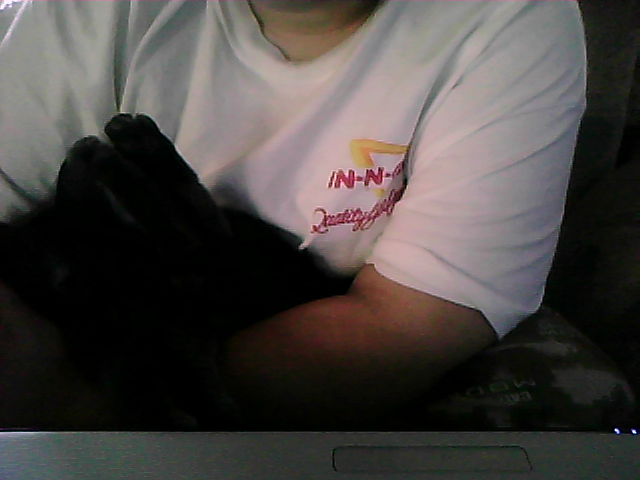
\includegraphics[width=0.5\textwidth]{original}
	\caption{Figure 1.1. Original image}
\end{figure}
\begin{figure}[h]
	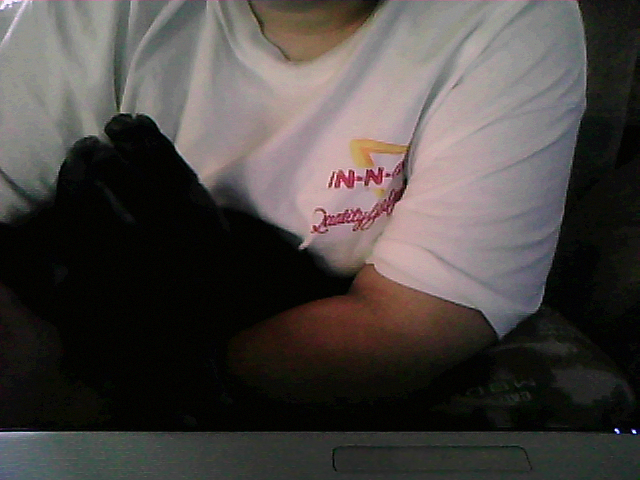
\includegraphics[width=0.5\textwidth]{modified}
	\caption{Figure 1.2. Image encoded with a xxx byte message}
\end{figure}
The VSL determined that there is a message about a xxx byte message in the original image. In reality, there is no message encoded into the original, but this value allows us to compare the two images. VSL determined that the modified image has a xxx byte message encoded into it. ADD VALUES AND FIX ANALYSIS Not only can steganalysis detected changes, but they are visually apparent as well. Figure 1.3 shows both an encoded image and its original.

\begin{figure}[h]
	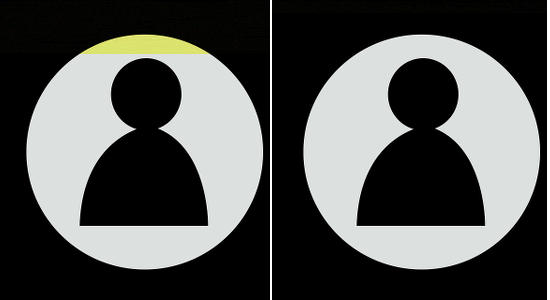
\includegraphics[width=0.5\textwidth]{comparison}
	\caption{Figure 1.3. Left: encoded, Right: original}
\end{figure}
The discoloration at the top of the encoded image is from the LSB encoding and this shows an obvious visual discoloration that an adversary can easily detect.

\subsubsection{Mitigating Risks of Steganography}
%Not enough data
These risks are mitigated by the fact that there is no universal standard for steganography methods. A user can easily replace the steganography module that we offer with a module of their own. That way, even if someone knows an image is not the original, that person will still not know who encoded it, or what kind of module was using for the encoding. Also, an encryption module can easily be added to our application and used to encrypt messages before they are encoded into an image. So even if someone knows what kind of steganography module is being used to encode messages into images, that person will also have the added challenge of decrypting the information. Although, there is no research to indicate that encryption helps in fooling steganalysis tools. Finally, since the original images exist on the internet, it will limit the plausible deniability of the user. It can be called into question as to why a certain user is uploading images that do not belong to that user to an online image database. 

%IMPLEMENTATION SECTION
\subsection{Encoding a File System}

The covert file system uses a drop in steganography module that takes in a bytearray object and returns a URL to an image. We used "least significant bit" steganography for this application because of its simplicity and reliability.

\subsubsection{Steganography Implementation}

Least significant bit (LSB) steganography is a Substitution type of steganography~\cite{Nosrati2011} that replaces the least significant bits in the image's pixels. Our steganography module is not true LSB steganography because we replace multiple bits in each pixel allowing us to encode one byte of data into every pixel. We designed our steganography technique this way to decrease the amount of images required to encode large file systems at the cost of only minimal discoloring. 

First, we break every byte of the message into three segments. Two segments of the byte will contain three bits, and the last segment will contain two bits. Next, we replace the three least significant bits of the red component with the first three bit segment. The green component follows, with the replacement of its least significant bits with the second three bit segment. Lastly, we replace the two least significant bits of the blue component with the remaining two bit segment of data. 

There are obvious drawbacks to our implementation of LSB steganography, primarily that the image may appear distorted as seen in Figure X and CovertFS images are X percent easier to detect using standard statistical analysis techniques compared to true LSB steganography as seen in figure X. However, this implementation enables us to store more bytes than other implementations of LSB steganography which decreases the latency in uploading and downloading images in large file systems [? Need evidence].
 
\subsubsection{File System to Images}

%David, I will need you to describe how the FUSE file system is prepared for encoding. Additionally, I will need information on how the files are uploaded as they are added to the file system (and future parallel upload/download). 
The first step in encoding a file system is retrieving an image. We use "The Cat API" which retrieves a random cat picture from Tumblr [?]. Once we retrieve the image, we determine the number of bytes we can encode in the image by multiplying the height and width of the image, in pixels. Since we encode one byte per pixel, the result of height times width results in the total number of bytes, \textit{n}, of data we can encode in the image. For example, a 640x480 pixel image can hold 307,200 bytes of data. Next, we take the data we are going to encode and append a special end of file byte encoding. Then, we break the data into two sets, one containing the last \textit{n} bytes and the other the remaining bytes. 

Next, we encode the data in the first set into the image and upload the image. We retrieve the URL of the uploaded image and append a URL identifier byte encoding along with the URL itself to the remaining data. Then, we repeat the encoding steps by appending the end of file byte encoding, splitting the data, and uploading until there is no data left to encode. At this point, we have encoded all the data and have a "linked list" of encoded images containing the data. Finally, we can return the URL to the head image of data. 
